\chapter{Metodologia}
  \section{Gerenciamento}
    \subsection{Estrutura Analítica do Projeto (EAP)}

      Tendo como objetivo a visão geral sobre as atividades que serão
      realizadas no decorrer do projeto, escolheu-se a EAP como forma
      de organização sistematizada das informações.

      A EAP consiste em uma organização das entregas
      a serem feitas em um formato de árvore, partindo de tarefas
      mais gerais para tarefas mais específicas \cite{pmbok2012}.

      Para a construção da EAP, foram levados em conta as diferentes
      entregas de pacotes a serem realizadas dentro do ciclo de vida do projeto,
      assim como as áreas de atuação dentro da equipe. Além disso, é
      possível observar o alinhamento da EAP com as atividades previstas, no caso o pacote de trabalho, e com os requisitos estabelecidos para o projeto.

      A figura \ref{fig:eap} é a representação gráfica da EAP do projeto.

      \begin{figure}[!htbp]
        \centering
        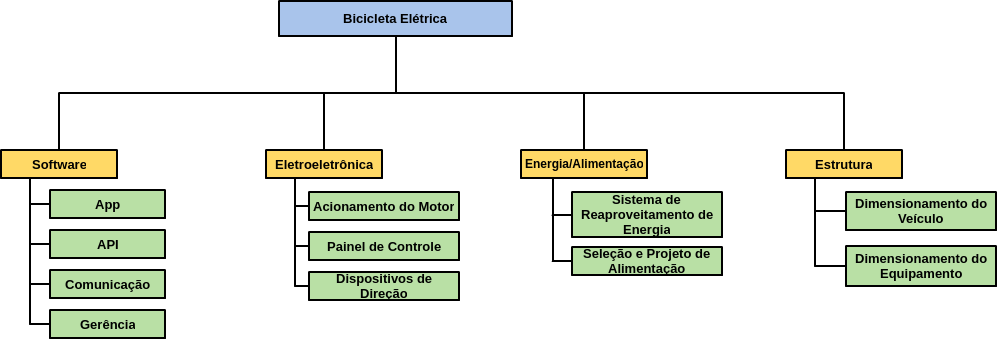
\includegraphics[width=\textwidth]{figuras/Eap.png}
        \caption{Estrutura Analítica do Projeto. Fonte: autores.}
        \label{fig:eap}
      \end{figure}

      \vfill
      \pagebreak

	\subsection{Plano de Riscos}
	\textbf{Objetivos}
		Este documento tem como finalidade estabelecer um processo de gerenciamento de riscos que podem vir a acontecer no projeto e a identificação dos mesmos pela equipe.
		
		\textbf{Descrição dos processos de gerenciamento de riscos}
		O Plano de Gerenciamento de Riscos contém seus processos definidos em quatro abordagens específicas segundo Max \cite{wideman1992project}. Sendo que todas as abordagens são necessárias pois elas se complementam para gerenciamento todas elas foram adotadas, sendo elas:
		
		\graphicspath{{figuras/}}
		\begin{figure}[h]
			\centering
			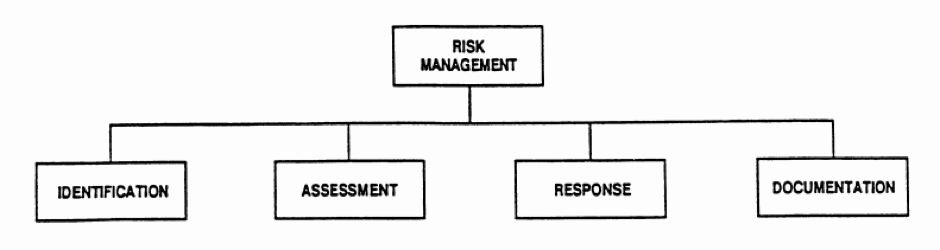
\includegraphics[scale=0.80]{EAP_Gerenciamento_de_Riscos.png}
			\caption{Etapas do plano de gerenciamento de riscos segundo Max \cite{wideman1992project}}
			\label{img:eap_gerenciamento_de_risco}
		\end{figure}
		
		\begin{itemize}
			\item \textbf{Identificação}: Esta fase consiste em identificar todos os possíveis riscos que podem impactar de forma severa o sucesso do projeto. Os tipos de impacto podem variar dependendo de onde ele afeta no projeto e quais as probabilidades deles acontecerem. Combinações de riscos que juntos podem representar uma ameaça mais do que individualmente não podem ser ignorados.
			\item \textbf{Avaliação}: Tendo identificado todo o alcance de riscos possíveis o próximo passo é os avaliar. O propósito é determinar os atributos do erro como o impacto, probabilidade e tipo de erro.
			\item \textbf{Resposta}: A parte de mitigação de riscos no projeto consiste em estabelecer uma estratégia de sistema apropriada, assim garantindo uma abordagem apropriada aos riscos caso eles venham a acontecer. Nesta etapa é descrito qual será a reação da equipe para tratar algum tipo de risco caso ele venha a acontecer.
			\item \textbf{Documentação}: Documento final e vital para o projeto que detalha todos os riscos, com suas características e quais serão as ações tomadas pela equipe de forma detalhada,caso cada risco apontado chegue a acontecer.
		\end{itemize}
		
		\textbf{EAR - Estrutura Analítica de Riscos para identificação dos riscos}
		O Project Management Institute (PMI), instituto que elaborou o Project Management Book of Knowledge (PMBoK) \cite{pmbok2012}, possui um template de estrutura analitica de riscos que possui as seguintes categorias e sub-divisões: 
		
		\graphicspath{{figuras/}}
		\begin{figure}[h!]
			\centering
			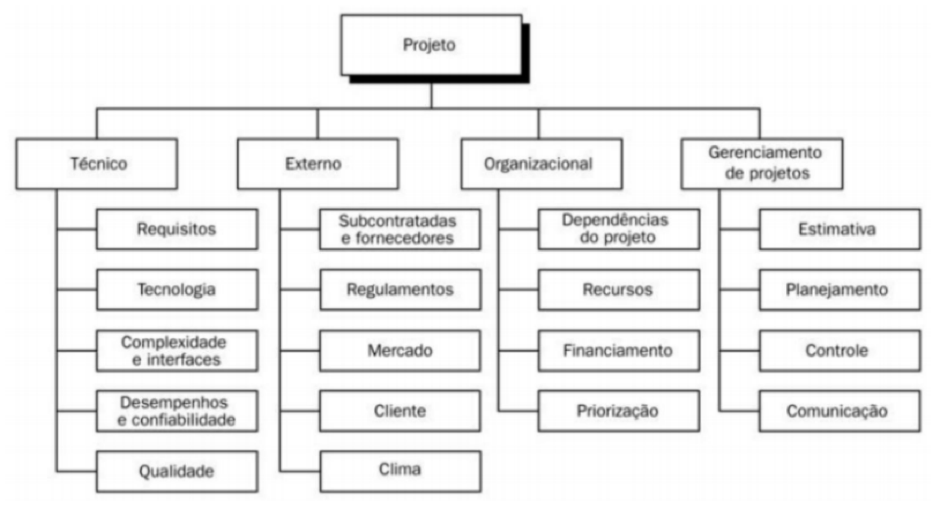
\includegraphics[scale=0.80]{classificacao_de_riscos.png}
			\caption{Classificação dos riscos na EAR segundo o PMI}
			\label{img:classificacao_de_riscos}
		\end{figure}
		
		\graphicspath{{figuras/}}
		\begin{figure}[h!]
			\centering
			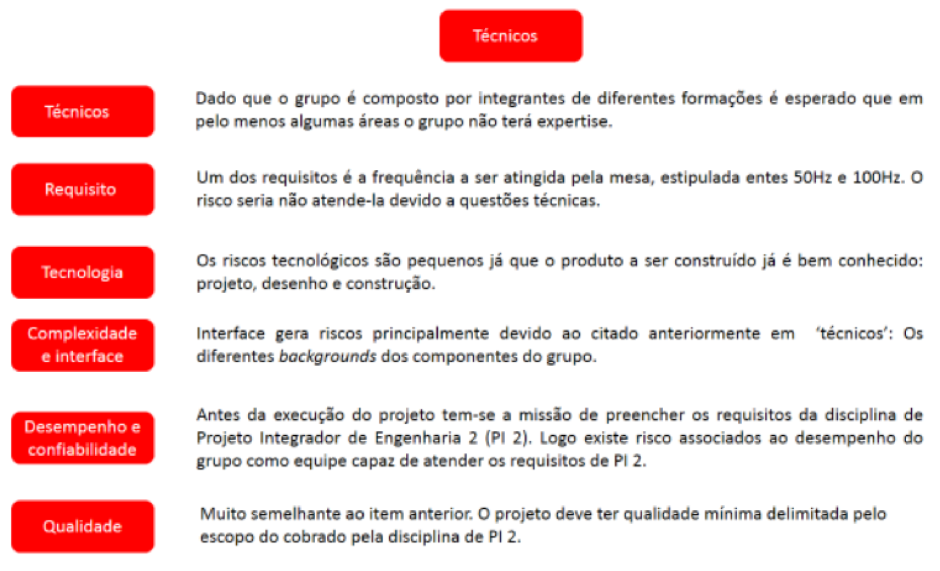
\includegraphics[scale=0.80]{analise_riscos_tecnicos.png}
			\caption{Análise em relação aos riscos técnicos}
			\label{img:analise_riscos_tecnicos}
		\end{figure}
		
		\graphicspath{{figuras/}}
		\begin{figure}[h!]
			\centering
			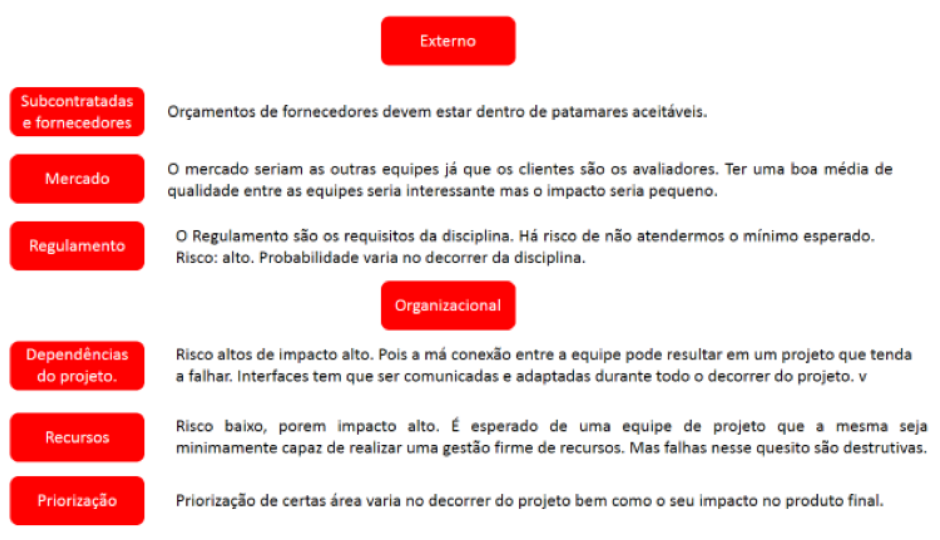
\includegraphics[scale=0.80]{analise_riscos_externos.png}
			\caption{Análise em relação aos riscos externos e organizacionais}
			\label{img:analise_riscos_externos}
		\end{figure}	
		
		\textbf{Qualificação dos Riscos}
		Os riscos identificados pelo grupo foram qualificados de acordo com sua probabilidade de ocorrência e o impacto resultante no projeto. O sistema de probabilidade e impactos foram classificados de acordo com a tabela padronizada do Gantter (ferramenta de gerenciamento de riscos adotada pela equipe).
		
		\begin{table}[h!]
			\centering
			\caption{Probabilidade dos Riscos}
			\label{tabela_probabilidade_riscos}
			\begin{tabular}{|ll|}
				\hline
				\multicolumn{1}{|l|}{\textbf{Nível}} & \textbf{Probabilidade} \\ \hline
				Improvável                           & 0\% $\sim$ 20\%        \\
				Remoto                               & 21\% $\sim$ 40\%       \\
				Ocasional                            & 41\% $\sim$ 60\%       \\
				Provável                             & 61\% $\sim$ 80\%       \\
				Frequente                            & 81\% $\sim$ 100\%      \\ \hline
			\end{tabular}
		\end{table}	
		
		\begin{table}[h!]
			\centering
			\caption{Severidade dos Riscos}
			\label{tabela_severidade_de_riscos}
			\begin{tabular}{|ll|}
				\hline
				\multicolumn{1}{|l|}{\textbf{Nível}} & \textbf{Descrição}                                                                                                                                                             \\ \hline
				Negligível                           & Risco que não afeta a integridade do projeto de forma a comprometer o mesmo.                                                                                                   \\ \hline
				Baixo                                & Possui pouco prejuízo ao desenvolvimento do projeto.                                                                                                                           \\ \hline
				Moderado                             & \begin{tabular}[c]{@{}l@{}}Prejudica o desenvolvimento do projeto. Pode ser resolvido\\ em um curto período de tempo.\end{tabular}                                             \\ \hline
				Significante                         & \begin{tabular}[c]{@{}l@{}}Prejudica o desenvolvimento do projeto. Gasta-se um tempo significativo\\ (semanas) para conseguir restituir a integridade do projeto.\end{tabular} \\ \hline
				Catastrófico                         & Erro que previne o projeto de ser concluído.                                                                                                                                   \\ \hline
			\end{tabular}
		\end{table}
		
		\textbf{Prioridade dos Riscos}
		A prioridade dos riscos também foi feita de acordo com as opções já padronizadas da ferramenta “Gantter”, sendo elas:
		
		\begin{table}[h!]
			\centering
			\caption{Prioridade dos Riscos}
			\label{tabela_prioridade_dos_riscos}
			\begin{tabular}{|ll|}
				\hline
				\multicolumn{1}{|l|}{\textbf{Nível}} & \textbf{Descrição}                                                                                                                                                                                                                  \\ \hline
				Sem Ação                             & O risco é tão pequeno ou irrelevante que nenhuma ação será tomada.                                                                                                                                                                  \\ \hline
				Monitorar                            & \begin{tabular}[c]{@{}l@{}}O risco possui um certo grau de causar problemas, sendo \\ monitorado constantemente.\end{tabular}                                                                                                       \\ \hline
				Tomar Ação                           & \begin{tabular}[c]{@{}l@{}}O risco possui uma boa probabilidade de causar problemas no projeto \\ e devem ser tomadas medidas de mitigação para que o mesmo não \\ aconteça ou reduza seu impacto.\end{tabular}                     \\ \hline
				Ação Urgente                         & \begin{tabular}[c]{@{}l@{}}O risco possui uma boa probabilidade de causar muitos problemas no \\ projeto e devem ser tomadas medidas prioritárias de mitigação para que\\  o mesmo não aconteça ou reduza seu impacto.\end{tabular} \\ \hline
				Interromper Projeto                  & \begin{tabular}[c]{@{}l@{}}O risco é tão significante que se interrompe o projeto até que seja \\ encontrada uma forma de contornar tal erro.\end{tabular}                                                                          \\ \hline
			\end{tabular}
		\end{table}	
		
		\textbf{Riscos Identificados}
		Os riscos identificados para o projeto estão listados na Tabela \ref{riscos_identificados}
		
		\begin{table}[h!]
			\centering
			\caption{Riscos Identificados}
			\label{riscos_identificados}
			\begin{tabular}{|llll|}
				\hline
				\multicolumn{1}{|l|}{\textbf{Risco}}       & \multicolumn{1}{l|}{\textbf{Probabilidade}} & \multicolumn{1}{l|}{\textbf{Severidade}} & \textbf{Prioridade} \\ \hline
				Trancamento de um integrante do grupo      & Remoto                                      & Moderada                                 & Monitorar           \\ \hline
				Atraso nas entregas das atividades         & Provável                                    & Significante                             & Ação Urgente        \\ \hline
				Desentendimento entre os membros da equipe & Ocasional                                   & Baixa                                    & Monitorar           \\ \hline
				Atraso na entrega de um produto/serviço    & Ocasional                                   & Significante                             & Ação Urgente        \\ \hline
				Problemas com a API                        & Remoto                                      & Catastrófica                             & Ação Urgente        \\ \hline
				Vibração do motor                          & Remoto                                      & Baixa                                    & Monitorar           \\ \hline
				Aquecimento dos componentes                & Remoto                                      & Moderada                                 & Monitorar           \\ \hline
				Ergonomia do produto                       & Remoto                                      & Baixa                                    & Monitorar           \\ \hline
				Custo inviável                             & Remoto                                      & Significante                             & Monitorar           \\ \hline
				Atraso/falta dos integrantes nas reuniões  & Remoto                                      & Moderada                                 & Tomar Ação          \\ \hline
			\end{tabular}
		\end{table}
		
		\textbf{Ação de Resposta aos Riscos}
		As ações que foram definidas pelo time à serem tomadas para cada risco identificado se encontram na Tabela \ref{acoes_de_resposta}.
		
		\begin{table}[!h]
			\centering
			\caption{Ações de Respostas aos Riscos}
			\label{acoes_de_resposta}
			\begin{tabular}{|ll|}
				\hline
				\multicolumn{1}{|l|}{\textbf{Risco}}       & \textbf{Resposta}                                                                                        \\ \hline
				Trancamento de um integrante do grupo      & \begin{tabular}[c]{@{}l@{}}Redistribuir as atividades entre os \\ membros da mesma equipe\end{tabular}   \\ \hline
				Atraso nas entregas das atividades         & \begin{tabular}[c]{@{}l@{}}Realinhar o cronograma e atuação do \\ responsável por tal grupo\end{tabular} \\ \hline
				Desentendimento entre os membros da equipe & Alinhamento de idéias através dos líderes                                                                \\ \hline
				Atraso na entrega de um produto/serviço    & \begin{tabular}[c]{@{}l@{}}Reunião dos líderes e tomada de ação no \\ setor com problemas\end{tabular}   \\ \hline
				Problemas com a API                        & Procurar uma nova API                                                                                    \\ \hline
				Vibração do motor                          & Procurar uma solução melhor                                                                              \\ \hline
				Aquecimento dos componentes                & Replanejamento da estrutura                                                                              \\ \hline
				Ergonomia do produto                       & Replanejamento da estrutura                                                                              \\ \hline
				Custo inviável                             & Replanejamento dos componentes                                                                           \\ \hline
				Atraso/falta dos integrantes nas reuniões  & \begin{tabular}[c]{@{}l@{}}Comunicação entre os representantes do \\ grupo com o indivíduo\end{tabular}  \\ \hline
			\end{tabular}
		\end{table}
		
		\textbf{Sistema de Controle de Mudanças de Riscos}
		O sistema serve justamente para alinhar a equipe sobre os riscos que o projeto pode vir a ter em seu decorrer e quais serão as ações que devem ser tomadas para cada tipo. A equipe deve estar consciente da probabilidade de cada risco encontrado a fim de controlar e manter o progresso do projeto em um meio que o risco possa sempre ser evitado.
		
		Cada risco não encontrado pelo grupo na fase de elaboração do projeto deverá ser documentado neste documento no futuro segundo os padrões adotados pela equipe e da ferramenta usada por ela para gerenciamento de riscos.

    \subsection{Plano de Recursos Humanos}
	Para este projeto foram designados treze alunos de cinco cursos de engenharia da Universidade de Brasília. Os alunos foram escolhidos dos cursos de Engenharia Aeroespacial, Engenharia Automotiva, Engenharia Eletrônica, Engenharia de Energia e Engenharia de Softwre. Com base nas engenharias foi dividido o trabalho em quatro frentes de atuação sendo elas:
	\begin{itemize}
		\item \textbf{Software}: responsável pela implementação do aplicativo e comunicação com os microcontroladores.
		\item \textbf{Eletroeletrônica}: responsável pela implementação dos microcontroladores e acionamento do motor.
		\item \textbf{Alimentação}: responsável por todo suprimento energético.
		\item \textbf{Estrutura}: responsável por desenhar e elaborar a estrutura do veículo.
	\end{itemize}
	
	A figura \ref{img:projeto} apresenta as áreas de trabalho com os seus integrantes. Os integrantes foram alocados de acordo com a especialidade e conhecimento adquirido durante o curso de graduação.
	
	\graphicspath{{figuras/}}
	\begin{figure}[h!]
	\centering
	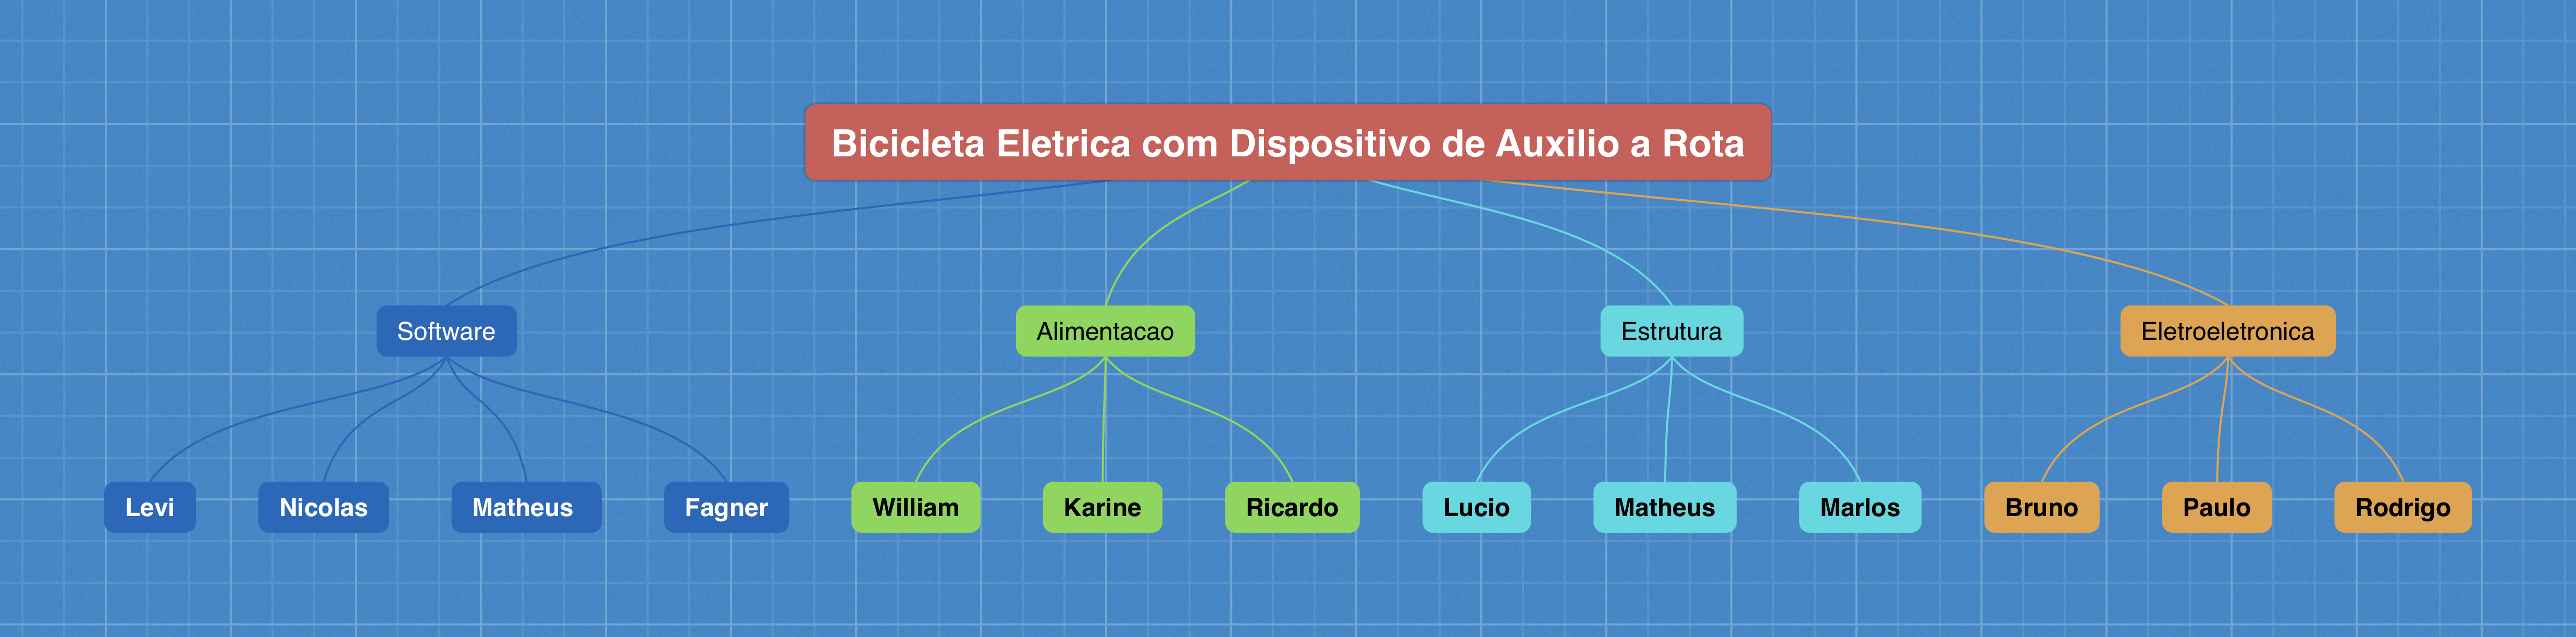
\includegraphics[scale=0.20]{project.png}
	\caption{Áreas de desenvolvimento e seus respectivos integrantes}
	\label{img:projeto}
	\end{figure}


    \subsection{Plano de Comunicação}

      Para que qualquer projeto tenha sucesso é necessário o engajamento da equipe, sendo assim, é necessário uma comunicação eficaz entre os membros da equipe. A tabela \ref{tab:com} detalha os métodos de comunicação utilizados pela equipe.
      
      \begin{table}[!htbp]
      	\begin{center}
      		\caption{\label{tab:com}Métodos de comunicação. Fonte: autores.}
      		\begin{tabular}{|p{4cm}|p{4cm}|p{3cm}|p{3cm}|p{2cm}|}
      			\hline
      			\textbf{Objetivos} & \textbf{Ferramenta} & \textbf{Frequência} & \textbf{Horário} & \textbf{Local}\\\hline\hline
      			Acompanhamento das atividades & Kanban & Sob demanda & Horário da disciplina & FGA\\\hline
      			Avisos rápidos / Lembretes & Telegram & Sob demanda & N/A & N/A\\\hline
      			Decisões Técnicas/Planejamentos & Presencial & Duas vezes por semana & Horário da disciplina & FGA\\\hline
      			Desenvolvimento do projeto & Google Docs/ Google Hangouts/ Git / Github / Presencial & Sob demanda & Durante desenvolvimento do projeto & N/A\\\hline
      		\end{tabular}
      	\end{center}
      \end{table}

\newpage

    \subsection{Plano de Tempo}
	O cronograma serve como uma ferramenta de gerenciamento do tempo, onde são colocados datas de início e término das atividades. Neste tópico é apresentado uma versão completa de como foi organizado o cronograma para gerenciamento do tempo do grupo. Um cronograma contendo o detalhamento das atividades é apresentado no apendice deste documento.

	Como é possível ver na figura \ref{img:cronograma_geral}, o projeto foi dividido em 3 grandes marcos (Pontos de Controle). As atividades se alinharam de acordo com o que é esperado em cada marco. No primeiro marco, as entregas são focadas na definição das tecnologias e na forma como será elaborado o produto final. O segundo marco tem como objetivo, a implementação do produto específico de cada área de conhecimento (Alimentação, Software, Estrutura e Eletroeletrônica). Ao fim do terceiro e último marco, espera-se que todas as áreas sejam capazes de integrar o produto desenvolvido no marco 2. 

	\graphicspath{{figuras/}}
	\begin{figure}[h!]
	\centering
	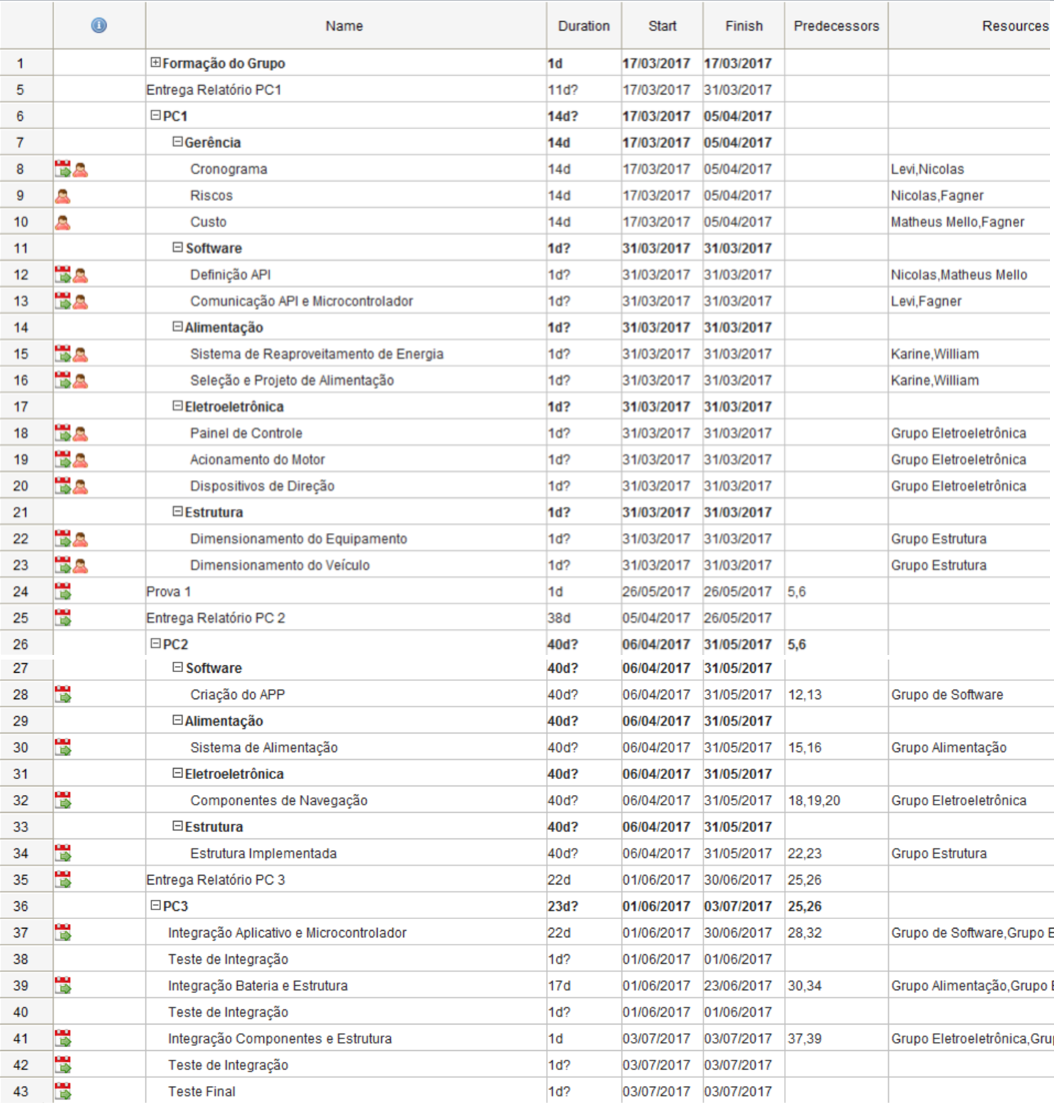
\includegraphics[scale=0.80]{cronograma_geral}
	\caption{Cronograma geral do projeto}
	\label{img:cronograma_geral}
	\end{figure}
	
	\newpage
	
	\textbf{Detalhamento do Cronograma}
	
		\textbf{Ponto de Controle 1}
		
		As atividades do Ponto de Controle 1 estão representadas na figura \ref{img:PC1}. As atividades foram divididas em cinco subgrupos que são:
		
		\begin{itemize}
			\item Gerência;
			\item Software;
			\item Alimentação;
			\item Eletroeletrônica;
			\item Estrutura;
		\end{itemize}	
		
		\graphicspath{{figuras/}}
		\begin{figure}[h!]
			\centering
			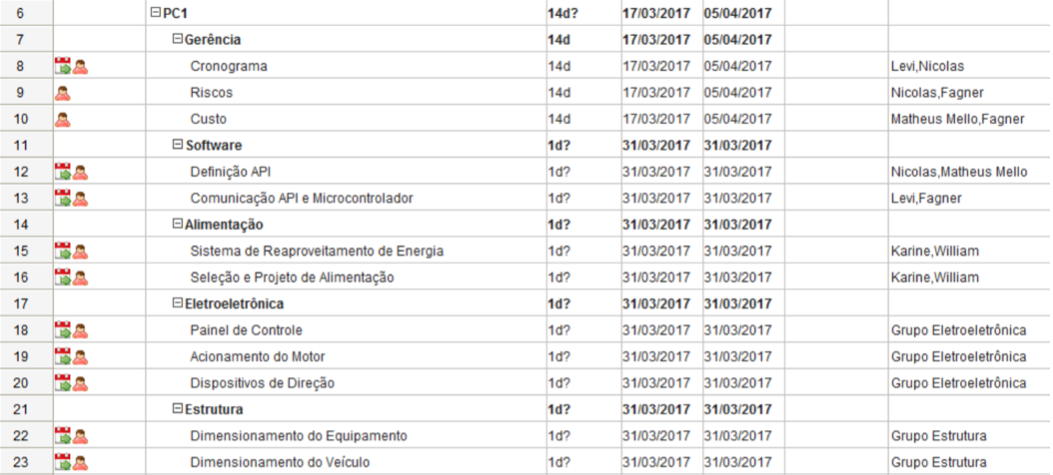
\includegraphics[scale=0.60]{PC1}
			\caption{Atividades do Ponto de Controle 1}
			\label{img:PC1}
		\end{figure}	
		
		As atividades do subgrupo de Gerência são:
		
		\begin{itemize}
			\item \textbf{Cronograma}: criação de um cronograma, contendo as datas de início e fim das atividades e os seus respectivos responsáveis.
			\item \textbf{Riscos}: definição dos riscos do projeto.
			\item \textbf{Custo}: levantamento dos custo do projeto, definindo a prioridade de aquisição.
		\end{itemize}	
		
		As atividades do subgrupo de Software são:
		
		\begin{itemize}
			\item \textbf{Definição API}: definir qual API será utilizada para implementação da solução de software.
			\item \textbf{Comunicação API e Microcontrolador}: definir a forma mais viável de transferir as informações coletadas pela API para o microcontrolador.
		\end{itemize}				
		
		As atividades do subgrupo de Alimentação são:
		
		\begin{itemize}
			\item \textbf{Sistema de Reaproveitamento de Energia}: definir um mecanismo que possa ser reaproveitar a energia e utiliza-lá para alimentação dos componentes eletrônicos.
			\item \textbf{Seleção e Projeto de Alimentação}: definir a melhor solução para alimentar o sistema. 
		\end{itemize}		
		
		As atividades do subgrupo de Eletroeletrônica são:
		\begin{itemize}
			\item \textbf{Painel de Controle}: definir o funcionamento do painél de controle acoplado à bicicleta para que se tenha informações do sistema.
			\item \textbf{Acionamento do Motor}: definir como será feito o acionamento do motor utilizando componentes eletrônicos.
			\item \textbf{Dispositivos de Direção}: definir os dispositivos de navegação que serão utilizados juntamente com a API de direção.
		\end{itemize}
		
		As atividades do subgrupo de Estrutura são:
		\begin{itemize}
			\item \textbf{Dimensionamento do Equipamento}: definir como serão acoplados os componentes eletrônicos ao sistema.
			\item \textbf{Dimensionamento do Veículo}: definir o desenho do veículo.
		\end{itemize}
		
		\textbf{Ponto de Controle 2}
		As atividades do Ponto de Controle 2 estão representadas na figura \ref{img:PC2}. As atividades foram divididas em quatro subgrupos que são:
		
		\begin{itemize}
			\item Software;
			\item Alimentação;
			\item Eletroeletrônica;
			\item Estrutura;
		\end{itemize}	
		
		\graphicspath{{figuras/}}
		\begin{figure}[h!]
			\centering
			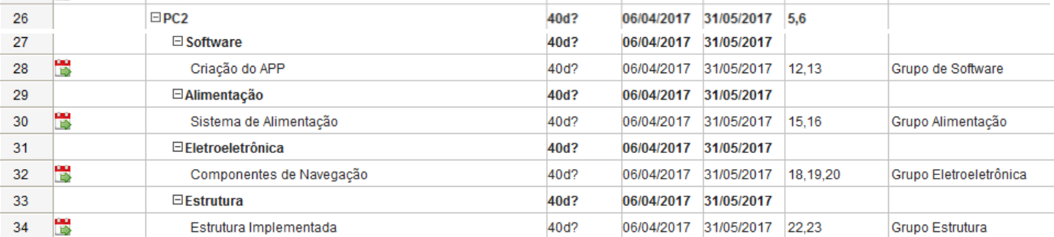
\includegraphics[scale=0.60]{PC2}
			\caption{Atividades do Ponto de Controle 2}
			\label{img:PC2}
		\end{figure}	
		
		As atividades do subgrupo de Software são:
		
		\begin{itemize}
			\item \textbf{Criação do APP}: implementar o app que fará a comunicação com o microcontrolador
		\end{itemize}
		
		As atividades do subgrupo de Alimentação são:
		\begin{itemize}
			\item \textbf{Sistema de Alimentação}: implementar o sistema que alimentará o veículo.
		\end{itemize}
		
		As atividades do subgrupo de Eletroeletrônica são:
		\begin{itemize}
			\item \textbf{Componentes de Navegação}: implementar o sistema de navegação que será acoplado ao veículo
		\end{itemize}
		
		As atividades do subgrupo de Estrutura são:
		\begin{itemize}
			\item \textbf{Estrutura Implementada}: implementar a estrutura do veículo.
		\end{itemize}
		
		\textbf{Ponto de Controle 3}
		As atividades do Ponto de Controle 2 estão representadas na figura \ref{img:PC3}.
		
		\graphicspath{{figuras/}}
		\begin{figure}[h!]
			\centering
			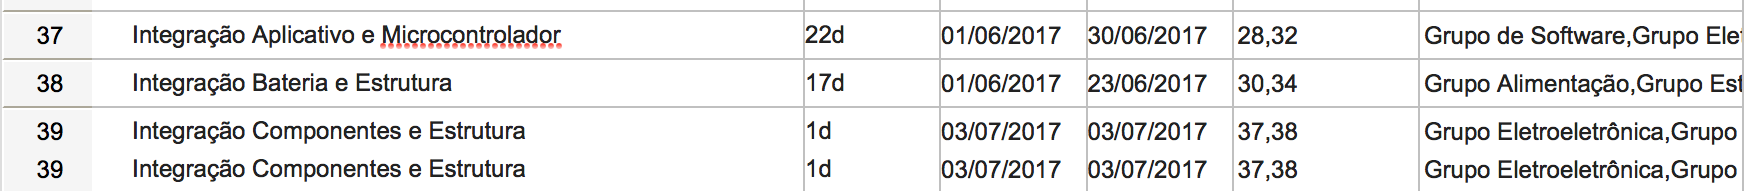
\includegraphics[scale=0.60]{PC3}
			\caption{Atividades do Ponto de Controle 3}
			\label{img:PC3}
		\end{figure}
		
		As atividades são:
		
		\begin{itemize}
			\item \textbf{Integração Aplicativo e Microcontrolador}: fazer a integração das duas interfaces e garantir o funcionamento do sistema.
			\item \textbf{Integração Bateria e Estrutura}: fazer o acoplamento da bateria à estrutura e garantir o funcionamento do sistema.
			\item \textbf{Integração Componentes e Estrutura}: fazer o acoplamento final entre os componentes e a estrutura (que já se encontra com a bateria), e garantir o funcionamento do sistema.
			\item \textbf{Teste de Integração}: teste que é feito ao fim de cada integração para garantir o funcionamento do sistema.
			\item \textbf{Teste Final}: teste feito ao fim de todas as integrações, onde o produto já foi finalizado. 
		\end{itemize}	
	
	\subsection{Plano de Custos}
	Para o planejamento de custos foi realizado uma estimativa inicial dos valores comerciais dos ingredientes necessários para o projeto pelo grupo. A partir daí, com base no valor total de todos os componentes, foi realizado uma divisão de uma valor exato para cada membro do grupo afim de já obter um caixa inicial para aquisições dos componentes. Ao final do projeto, a sobra do valor total será dividida e repassada aos componentes do grupo.
	
	A seguir pode-se verificar a tabela de custos para o projeto.
	
	\begin{table}[!htbp]
		\begin{center}
			\caption{\label{tab:custos}Custos iniciais.}
			\resizebox{\textwidth}{!}{
				\begin{tabular}{|p{4cm}|p{4cm}|p{3cm}|p{4cm}|}
					\hline
					\textbf{Material} & \textbf{Preço} & \textbf{Quantidade} & \textbf{Total}\\\hline\hline
					Motor 350W 36V & Cedido & 1 & R\$ 0,00\\\hline
					Celular Android & Cedido & 1 & R\$ 0,00\\\hline
					Bateria 12V 12Ah & R\$ 150,00 & 3 & R\$ 450,00 \\\hline
					Bateria 12V 1.3Ah & Cedido & 1 & R\$ 0,00 \\\hline
					Dínamo & R\$ 50,00 & 1 & R\$ 50,00 \\\hline
					Display LCD & R\$ 60,00 & 2 & R\$ 120,00 \\\hline
					Microcontrolador Arduíno & Cedido & 1 & R\$ 0,00 \\\hline
					Microprocessador MSP & Cedido & 1 & R\$ 0,00 \\\hline
					Placa de Cobre & R\$ 15,00 & 1 & R\$ 15,00 \\\hline
					Rolo de Estanho & R\$ 30,00 & 1 & R\$ 30,00 \\\hline
					Ferro de Solda & Cedido & 1 & R\$ 0,00 \\\hline
					Componentes Eletrônicos & R\$ 30.00 & 1 & R\$ 30,00 \\\hline
					Selim Carbonado com Duas Molas MTB Kalf & R\$ 25,90 & 1 & R\$ 25,90 \\\hline
					Cabo de Aço para Freio de Bicicleta & R\$ 4.00 & 2 & R\$ 8,00 \\\hline
					Garfo 26 MTB 325 Aço Preto c/ Suspensão 21.1 Zoom & R\$ 92,90 & 1 & R\$ 92,90 \\\hline
					Guidão Downhill Aço Preto 580 mm & R\$ 8,90 & 1 & R\$ 8,90 \\\hline
					Jogo de 36 raios Inox & R\$ 78,00 & 2 & R\$ 156,00 \\\hline
					Pedal para Bicicleta MTB Alumínio Polido Prata 9/16 & R\$ 23,90 & 2 & R\$ 47,80 \\\hline
					Pneu 26x1.95 K.816 Preto Cravado & R\$ 101,80 & 2 & R\$ 203,60 \\\hline
					Roda Dentada 46 Dentes Aço Preto & R\$ 7,90 & 1 & R\$ 7,90 \\\hline
					Suporte de Guidão MTB 25.4mm Aço Preto & R\$ 15,90 & 1 & R\$ 15,90 \\\hline
					Freio V-brake Alumínio Preto com Maçaneta Completo & R\$ 51,90 & 1 & R\$ 51,90 \\\hline
					Pedivela Monobloco Preto 165x16mm Preto & R\$ 14,90 & 1 & R\$ 14,90 \\\hline
					Aro Aero com Folha Dupla de Alumínio 16 pol com Ilhós & R\$ 38,00 & 2 & R\$ 76,00 \\\hline
					Canote Selim Alumínio 26.8x290mm & R\$ 14,00 & 1 & R\$ 14,00 \\\hline
					Câmara de Ar & R\$ 30,00 & 2 & R\$ 60,00 \\\hline\hline
					\textbf{Custo Total} & - & - & R\$ 1.478,70 \\\hline
				\end{tabular}
			}
		\end{center}
	\end{table}